%allowed: 6 pages + 1 page for references
%blind submission

% to include comments in the generated pdf comment the \commfalse and uncomment \commtrue
\newif\ifcomm
\commtrue
%https://www.sharelatex.com/project/5a3bd322e005042d729dbbc5
%\commfalse

% to produce the double-blind paper version comment the \blindfalse uncomment the \blindtrue
\newif\ifblind
\blindtrue
%\blindfalse


%%%%%%%%% From hotnets17.tex %%%%%%%%%%%

\documentclass{hotnets17}

\usepackage{times}  
\usepackage{hyperref}
%\usepackage{color}
\usepackage[usenames, dvipsnames]{color}

\hypersetup{pdfstartview=FitH,pdfpagelayout=SinglePage}
\usepackage{hyperref}
\definecolor{darkred}{rgb}{0.7,0,0}
\definecolor{darkgreen}{rgb}{0,0.5,0}
\hypersetup{colorlinks=true,
        linkcolor=darkred,
        citecolor=darkgreen}
%\hypersetup{pdfstartview=FitH,pdfpagelayout=SinglePage}      
%  \def\UrlBreaks{\do\/\do-}
  \setlength{\parskip}{0pt}

\setlength\paperheight {11in}
\setlength\paperwidth {8.5in}
\setlength{\textwidth}{7in}
\setlength{\textheight}{9.25in}
\setlength{\oddsidemargin}{-.25in}
\setlength{\evensidemargin}{-.25in}

%%%%%%%%%%%%%%%%%%%%%%%%%%%%%%%%%%%%%%%%%%%%

\usepackage[utf8]{inputenc}
%\usepackage[numbers]{natbib}
\usepackage[noadjust]{cite}
%\renewcommand{\citedash}{--}  
\usepackage[inline]{enumitem}
\newlist{inlinelist}{enumerate*}{1}
\setlist[inlinelist]{label=(\arabic*)}
\newlist{romanlist}{enumerate*}{1}
\setlist[romanlist]{label=(\roman*)}

\usepackage[english]{babel}
\usepackage{times}
\usepackage{amsmath}
\usepackage{setspace}

\newtheorem{definition}{{\bf Definition}}
\newtheorem{proposition}{{\bf Proposition}}

%\usepackage{amsthm}
\usepackage{amsfonts}
%\usepackage{subfigure}
%\usepackage{stmaryrd}
%\usepackage{float}
\usepackage{graphicx}
\usepackage{caption}
\usepackage{subcaption}
\usepackage{textcomp}
\usepackage{xspace}

%\usepackage{algorithm}
%\usepackage{algorithmicx}
%\usepackage{algpseudocode}
%
%\input{aamas_defs}

%\usepackage{tikz}
%\usetikzlibrary{arrows,decorations,decorations.shapes,backgrounds,shapes}


\newtheorem{theorem}{Theorem}[section]
\newtheorem{corollary}[theorem]{Corollary}
\newtheorem{lemma}[theorem]{Lemma}
\newtheorem{claim}[theorem]{Claim}
\newtheorem{conjecture}[theorem]{Conjecture}

%\theoremstyle{definition}
\newtheorem{example}[theorem]{Example}
%\newtheorem{definition}[theorem]{Definition}
\newtheorem{remark}[theorem]{Remark}

\ifcomm
	\newcommand{\mycomm}[3]{{\color{#2} \textbf{[#1: #3]}}} 
\else
    \newcommand{\mycomm}[3]{}
\fi

%define your comment NAME and COLOR here
\newcommand{\IK}[1]{\mycomm{IK}{blue}{#1}}
\newcommand{\AB}[1]{\mycomm{AB}{Orange}{#1}}
\newcommand{\NR}[1]{\mycomm{NR}{OliveGreen}{#1}}
\newcommand{\MS}[1]{\mycomm{MS}{red}{#1}}
\newcommand{\EZ}[1]{\mycomm{EZ}{BlueGreen}{#1}}

\providecommand{\vs}{vs. }
\providecommand{\ie}{\emph{i.e.,} }
\providecommand{\eg}{\emph{e.g.,} }
\providecommand{\cf}{\emph{cf.,} }
\providecommand{\etc}{\emph{etc.} }

\def\compactify{\itemsep=0pt \topsep=0pt \partopsep=0pt \parsep=0pt}
  \let\latexusecounter=\usecounter
  \newenvironment{CompactItemize}
    {\def\usecounter{\compactify\latexusecounter}
     \begin{itemize}}
    {\end{itemize}\let\usecounter=\latexusecounter}
  \newenvironment{CompactEnumerate}
    {\def\usecounter{\compactify\latexusecounter}
     \begin{enumerate}}
    {\end{enumerate}\let\usecounter=\latexusecounter}
        
\newcommand{\T}[1]{\smallskip\noindent\textbf{#1}} %paragraph title
\newcommand{\U}[1]{\smallskip\noindent\textit{#1}} %paragraph sub-title
        

\newcommand{\newblock}{}

%a macro for defining a new variable in the document
\newcommand{\newVar}[2]{\newcommand{#1}{\ensuremath{#2}\xspace}}

%%%%%%%%%%%%%%%%%%%%%%%%%%%%%%%%%%%%%%%
\newVar{\rc}{R_C}
\newVar{\rs}{R_S}
\newVar{\rmid}{R_M}
\newVar{\rtt}{T}

\title{Cloudified Data Delivery: \\ It's the Congestion Control, Stupid! }

\author{} %blind
\date{}

\begin{document}

\maketitle
\sloppypar
    
\begin{abstract}
Data delivery through relays in the cloud is of quickly growing importance and is claimed to accelerate data transport. However, the reasons for this acceleration and the exact \textit{recipe} for optimizing performance remain little understood. We aim to quantify the potential of \textit{cloudified data delivery} and learn how to tap it. To this end, we explore the performance of different data transport strategies through hundreds of thousands of file downloads. 

Our results show that even simple strategies can improve file download times by an order of magnitude. A recurring theme in our results is that congestion control plays \emph{the} crucial role in achieving high performance. In fact, our results suggest that even \emph{routing} within the cloud should be oriented towards achieving better congestion control! We outline interesting and important directions for future research.
\end{abstract}

\section{Introduction}

Recently, schemes for data delivery through relays (virtual machines) in the cloud, which we refer to collectively as \emph{cloudified data delivery}, have been the subject of much attention in both academia and the industry~\cite{cgn2017,CRONets,wang2013accelerating,teridion,akamai}. \autoref{fig:overlay} illustrates the notion of cloudified data delivery, which spans a broad spectrum of scenarios, ranging from merely placing TCP proxies in the cloud~\cite{cgn2017} to deploying large-scale overlay networks and optimizing routing within the cloud~\cite{teridion,CRONets}.

% \autoref{fig:overlay} illustrates a simple 4-node cloud-based overlay network. Its nodes are virtual machines in the cloud placed at different geographic locations. These nodes can function as data transmission relays. %Lines between the relay nodes depict the (logical) links of the overlay network, each representing the underlying route between the relevant relays. 
% When user $A$ sends a packet to user $B$, instead of simply routing it on the default dashed E2E (end-to-end) BGP route, it can route it through a solid BGP route to cloud relay $R_A$ instead, which can forward it to cloud relay $R_B$ within the cloud. Finally, cloud relay $R_B$ forwards the packet to $B$ through a default BGP route.

\begin{figure}[t]
  \centering
    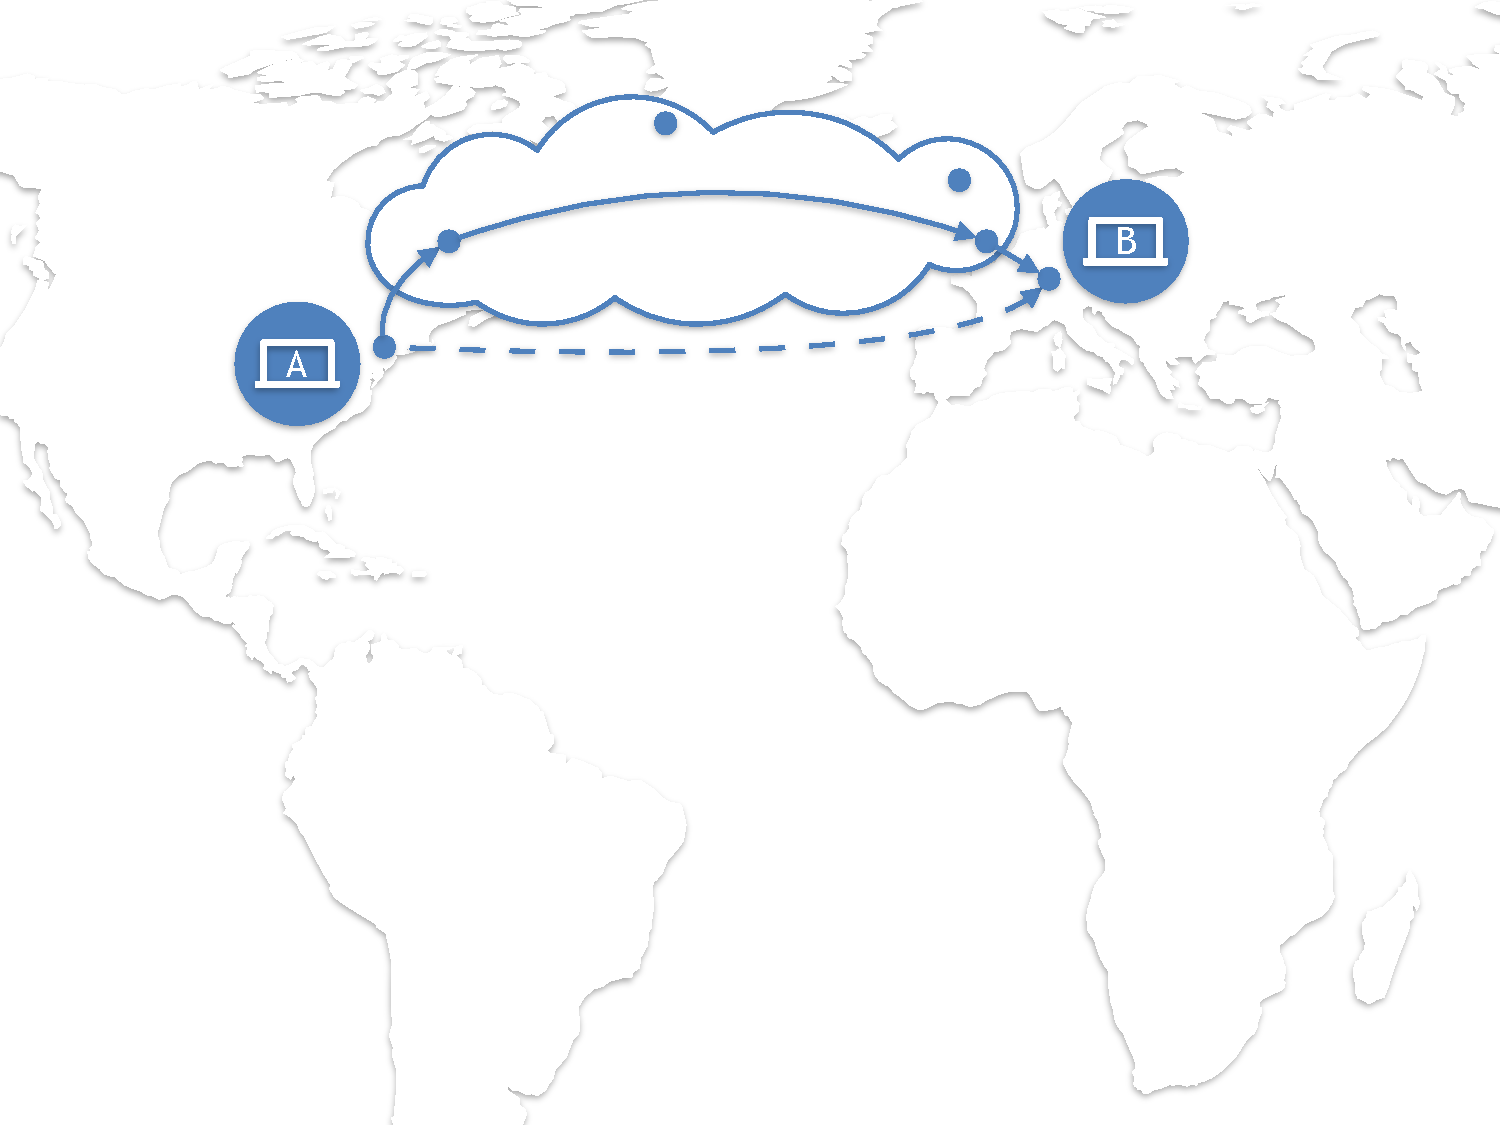
\includegraphics[width=\columnwidth]{figures/overlay-network}
    \caption{\textit{Cloudified data delivery} using a simple  4-node cloud-based overlay network. The nodes are virtual machines in the cloud placed at different geographic locations. They can function as data transmission relays. %Lines between the relay nodes depict the (logical) links of the overlay network, each representing the underlying route between the relevant relays. 
When user $A$ sends an IP packet to user $B$, instead of simply routing it on the default dashed E2E (end-to-end) BGP route, it can route it through a \textit{two-relay cloudified route}: first, a solid-line BGP route to cloud relay $R_A$, which forwards it within the cloud to cloud relay $R_B$, which  finally forwards it %. Finally, cloud relay $R_B$ forwards the packet 
to $B$ through a default BGP route. %\IK{[]Noga: I can make the following changes if you are too busy:] 1. Need to expand the caption 2. maybe cut the bottom half (south america+africa) 3. either add more lines to display a nice (but not full-mesh) topology, or correct the text, which mentions lines 4. give names to $R_1/R_A$ and $R_2/R_B$ to make the text easier? 5. can we place two relays on the path in the US?}
    }
    \label{fig:overlay}
\end{figure}

Recent studies~\cite{cgn2017,CRONets,wang2013accelerating} suggest that cloudified data delivery can accelerate data transport. However, the reasons for this acceleration and the exact \textit{recipe} for optimizing performance remain little understood. We believe that cloudified data delivery is still far from realizing its full potential and will play an important role in future paradigms for data delivery. Our aim is hence to \emph{quantify} its potential and learn how to tap it. In our quest for optimized cloudified data delivery, we seek answers to several questions: 
\begin{inlinelist}
    \item How many relays should be used? ($1$? $2$? $3$? more?)
    \item How important is \emph{optimizing} routing within the cloud?
    \item Should end-to-end congestion control between the communicating end-points be \emph{split} into multiple inter-hop connections?
    \item What is the effect of replacing TCP with more advanced congestion control schemes such as 
    \ifblind BBR~\cite{BBR}? \else
    PCC~\cite{PCC} and BBR~\cite{BBR}? \fi %in cloudified data delivery?
    \item Do different clouds differ in terms of performance benefits?
    \item Can significant benefits be derived from routes that traverse multiple different clouds? %(e.g., Amazon's, Google's, etc.), 
    %\item How does cloudified data delivery compare to simply using clever end-to-end congestion control?
\end{inlinelist}
%and more.

We take the first steps in this research direction. To evaluate the performance benefits of different routing and congestion control strategies for cloudified data delivery, we deployed relays on three major clouds: \textit{AWS} (Amazon web services), \textit{GCP} (Google cloud platform) and Microsoft \textit{Azure}. Within each cloud, we deployed nodes in all available regions  (14 in AWS, 10 in GCP, and 26 in Azure). We ran a total of some 380,000 file downloads, considering both inter-continental and intra-continental routing, with both large and small files, and with clients (traffic receivers) and servers (traffic senders) placed both within and outside the cloud. We measured performance in terms of file download completion time.

% \IK{the following paragraph is not entirely clear: maybe we should delete it? its first point is that we don't want to modify the end-points. If so, can we simply delete question (7) above? (or move it to future questions elsewhere, here it cuts the flow). Its second point runs against our last trial.}
% Our experiments are currently limited to the setting that the cloudified data delivery mechanism is in control of the relay nodes (as opposed to the clients and servers) and so do not (yet) address questions that involve, e.g., the end-points employing different congestion control protocols. Our experiments also do not capture routing traversing different clouds and so are currently limited to examining routing strategies \emph{within the same cloud} \EZ{still true?}. We discuss below our findings thus far.

We next present some of our main (preliminary) results. A recurring theme is that congestion control plays \emph{the} crucial role in achieving high performance.

\vspace{0.05in}\noindent{\bf Splitting end-to-end congestion control is a must.} Our experiments indicate that the \emph{most} crucial factor in attaining high performance is splitting the end-to-end congestion control connection into individual inter-hop connections. Indeed, without splitting the connection, routing through the cloud overlay does not lead to meaningful benefits (if any). Splitting thus seems like a \emph{necessary} condition for high performance. 

\vspace{0.05in}\noindent{\bf A simple routing strategy fares reasonably well.} We show that with TCP splitting, attaining reasonably high performance does not require sophisticated routing schemes. Specifically, the following two-relay routing strategy fares well: route traffic first to the cloud relay that is closest to the sender (both RTT-wise and location-wise work), then go through the relay that is closest to the receiver before sending the traffic to its destination. This captures the intuition that one need only enter the cloud as soon as possible and let the (highly optimized!~\cite{pretium,B4,one-hop,cgn2017,unusual,multidimensional}) cloud take care of the rest. 
%\NR{This next sentence I think is coming way too early - it has relay names and things not discussed yet. Can we remove it?}
For instance, an India-to-California large file transfer using TCP splitting and two relays on AWS %(in ap-so-1 and us-we-1) 
achieves a significant 5.89$\times$ improvement in file download time over default end-to-end transfer. Without TCP splitting, the improvement drops down to 1.4$\times$.  
%%%%%%This is mentioned again just below -- I remove it. (IK)
%---even though, while this scheme yields high performance,  we also find that it is not the \textit{best}. 
%We show that, while yielding high performance, this simple form of routing does not, in general, provide the \emph{best} performance guarantees.

\vspace{0.05in}\noindent{\bf This simple strategy is still suboptimal.} % not enough to tap the full potential of cloudified data delivery.} 
Our results show that while the above ``split TCP \& enter-close-and-exit-far'' approach achieves favorable performance, it is often suboptimal, in the sense that other strategies consistently provide better performance.  
%In particular, we find that selecting other routes within the cloud than those employed by our simple strategy often results in better performance.
In fact, instead of our simple two-relay strategy, even utilizing the best \emph{single} relay often yields better results (\eg in the India-California download, 6.64$\times$ when going through a relay in Singapore \vs 5.89$\times$ in the simple two-relay case). %---although the best single relay is only known in hindsight after trying all of them. 

This raises the question of how better performance should be attained. Interestingly, what is common to the better schemes identified by our experiments is that they are oriented towards 
%improving \emph{congestion control} performance within the cloud, not circumventing \emph{routing inefficiencies} within the cloud.
improving \emph{congestion control} performance, not circumventing \emph{routing inefficiencies}, within the cloud.

\vspace{0.05in}\noindent{\bf Approach (I): \textit{min-max-latency routing}.} %seek high-bandwidth routes within the cloud.}
A natural approach to finding good routes in the cloud is to look for routes with high available bandwidth. Unfortunately,
%Quick completion of large traffic flows crucially relies on the amount of available bandwidth, suggesting that clever routing within the cloud should seek paths with a lot of spare capacity. Unfortunately, 
the seemingly only way to \emph{accurately} quantify how much bandwidth is attainable on a certain route, is simply to fully utilize the available bandwidth, resulting in unreasonable costs. Indeed, common bandwidth-estimation approaches and tools are notoriously inaccurate~\cite{CRONets,tools}, and end-to-end latency also generally appears to be a bad indicator. 

%\vspace{0.05in}\noindent{\bf Approach II: min-max-latency routing!} 
While end-to-end latencies are not a good indicator of good performance, we develop a more sophisticated approach that also relies on measuring latencies, and thus avoids the obstacles associated with bandwidth estimation. %\AB{didn't get the last sentence}.
Specifically, consider the following strategy for cloudified data delivery. As in our simple strategy, routes through the cloud still enter the cloud via the relay $R_A$ that is close to the sender and leave via the relay $R_B$ that is close to the receiver. Unlike our simple strategy, traffic from $R_A$ to $R_B$ goes through an \emph{intermediate} relay $R_C$ within the cloud. The TCP connection between $R_A$ and $R_B$ is \textit{split} into the two segments $R_A \to R_C$ and $R_C \to R_B$. 
%\NR{What is $R_c$? This is the first time this term is being used, but it is not defined.}

The choice of $R_C$ will impact performance. How should it be chosen? Let $T({R_A \to R_C})$ and $T({R_C \to R_B})$ denote the two respective segment latencies.
%between $A$ and $C$, and between $C$ and $B$, respectively. 
We select $C$  to optimize the expression $\min\max\{T({R_A \to R_C}),T({R_C \to R_B})\}$, \ie the choice of $R_C$ is intended to minimize the worst-case latency between relays along the path $(R_A \to R_C \to R_B)$. This {practical} three-relay strategy consistently provides much better performance than the 2-relay strategy in our experiments. We hypothesize that this is not a result of identifying efficient routes, but of enabling TCP to ramp up its slow-start phase more quickly and to react faster (\eg to ACKs and packet losses) by reducing its response time. We refer to this strategy (which can be generalized to more relays) as \emph{min-max-latency routing}. (For example,  we get an 8.64$\times$ performance in the India-California file download with a min-max RTT of 123~ms. ) 
%\IK{Aran: does the min-max yield ap-ne-1 in Fig 3? I want to paste the number here. If so, we should state it there somewhere if we don't already.}\AB{Yes, it does. The max RTT for this route is 123 ms.}

\vspace{0.05in}\noindent{\bf Approach (II): \textit{Quick-Start TCP}.} Can similar performance benefits be attained without relying on optimizing routing within the overlay network? We show that this is achievable by using our \textit{simple} 
%\IK{should we call it ``baseline" instead of simple so people remember it when we refer to it here? note that I removed the word simple from the strategy above to prevent confusion} 
two-relay strategy \emph{and} initializing the congestion and flow control windows at the cloud relays to be very large, thus effectively skipping the slow-start~\cite{dukkipati2010}. Our experiments indicate that this approach effectively matches or surpasses the performance of min-max-latency routing, yielding the best (or near-best) observed performance (\eg an impressive 11.43$\times$ in the India-California file download). We refer to this strategy as \emph{Quick-Start TCP}.

Why is this happening? One hypothesis is that large windows induce aggression towards regular TCP connections sharing the same links/buffers, and that 
%; by skipping TCP's slow-start phase, 
this strategy is simply hogging the link for others. An opposing hypothesis is that bypassing TCP's slow-start enables connections to quickly take over unused capacity, thus making better use of the cloud's resources. Which is it then? The answer to this question should determine which of the two approaches--- min-max-latency or Quick-Start TCP --- is the most appropriate choice. We provide partial evidence that the latter hypothesis is correct.

\vspace{0.05in} To guarantee the reproducibility of our results and provide researchers with the ability to easily execute cloudified data delivery measurements, we intend to publish scripts that enable users to easily deploy virtual machines in the clouds and rerun our tests.

%\IK{What seems unique in our paper: (a) the first networking paper on the 3 major clouds??? (b) the first paper on aggressive within the cloud? (c) the first on 3 hops? (d) the first on hops in multiple clouds within the same path?}\AB{we have a single experiment with mixed clouds - still need to produce the graph for it.}

\section{Methodology}

%\IK{Important: can we tell them that they can play with something online? If not, can we promise them that there is some open-source code? Or even some VMs that they can download and run? Being able to replicate the results is important in this community, and the clouds help us  enable cool stuff.}
%\AB{I think we can publish the scripts we currently use (or a modified version of these scripts...) and add a README on how to run them. No need for a special VM. Just need to create VMs in the clouds (and we can also publish scripts for that).}


%% Moved to intro
% \IK{Maybe move this to the intro? We need to say sth like this somewhere.}
% In preparation for this paper, we ran of thousands of experiments \AB{actually - > 240K downloads by me and > 140K downloads by Noga. I don't know if I would call each an "experiment", though}, considering both inter-continental and intra-continental routing. For the sake of simplicity, we focus in this paper on representative examples, before discussing a few trends and outliers.
% international 
% . While not exhaustive by any means, they included various routing options: for example, West US to Mumbai via Asia, East US to Mumbai via Europe, and regional routing in Asia, Europe and the Americas. In the following chapters we discuss some of the trends observed, as well as outliers. 


\noindent{\bf Clouds.} We deployed relays (virtual machines) on three major clouds: \textit{AWS} (Amazon web services), \textit{GCP} (Google cloud platform) and Microsoft \textit{Azure}. In each cloud, we deployed one relay in each publicly-available region (\autoref{tab:cloud-config}), 
\begin{table}[t] {\small
    \centering 
    \begin{tabular}{c c c c}
        %\hline
         Cloud &            AWS &           Azure               & GCP \\ \hline %\hline
         \# of Regions &    14 &            26                  & 10 \\
         Machine %Type/Size 
            &     t2.micro &      Standard\_DS1\_v2   & n1-standard-1 \\
         \textcent/hour &   1.2 -- 2         & 7                 & 4.75 -- 6.74 \\
         \textcent/GB & 9  & 8.7 -- 18.1   & 12 -- 23 (1 in US) \\ \hline
       
        % \hline
    \end{tabular}
    \caption{Number of regions and machine types used in each cloud, and their pricing, taken from the cloud providers' website. 
    %\IK{I deleted lines to make it look nicer and compressed to fit single column; feel free to revert. Also, very minor: would the transpose of this table look better? Feel free to ignore.}
    }
    \label{tab:cloud-config}
    }
\end{table}
yielding a total of 50 relays. Each relay ran Ubuntu 17.04 using relatively cheap machine types. % \IK{simple machines}
%\AB{For the US experiments we used fewer regions -- we only used the regions the Americas. We should put that somewhere.}
%\NR{We actually deployed more than one VM per region, Aran has the total, but I'm guessing we had 100+ machines}
%\NR{@AB, you have the setup of all of the machines you deployed for both you and me, right?}\AB{For the Mumbai experiments I used all regions of the cloud provider tested. I.e., all 10 from GCP, 14 from AWS and 26 from Azure. For the US experiments I used the regions in America (i.e., all US regions and Canada and South America, if they exist for the particular cloud provider)}\NR{So, how do we want to fill this out?}
% \begin{romanlist}
%     \item AWS - 14 regions
%     \item GCP - 10 regions
%     \item Azure - 26 regions
% \end{romanlist}\AB{did we define these acronyms?}\NR{Nope, maybe it's a good place to do so}
% . 
%, and was used as either clients, relays, or servers\AB{So, will we have graphs were the VMs are used as servers? Do we want to call the VMs relays, Relays, Jump-hosts? Something else? (just to be consistent)}. \AB{I think that for this paper we should concentrate on clients and servers on the Internet (not the cloud), or at least - on a server on the Internet...}


\smallskip\noindent{\bf Servers.} We used two university-based servers: 
%For servers outside of the cloud, we have used to following: 
(1)~www.cc.iitb.ac.in, located in IIT Bombay, India; and (2)~www.college.columbia.edu, located in Columbia University, NY, US.
%The files from the first server were reused in the cloud servers. 
We chose university-based servers as these typically have fairly good Internet connection but do not use CDNs, and so download times are not expected to be affected by redirections or caching. We downloaded two types of files from these servers: large files (3.9~MB for the first server, 3.8~MB for the second), and small files (17~KB for the first server, 18~KB for the second).
%Our bandwidth tests relied on the large files. \AB{Do we need the last line?}

\smallskip\noindent{\bf Clients.} We used two types of clients: (1)~ a personal computer located in San Francisco (SF), connected to the Internet through Comcast; and (2)~PlanetLab~\cite{PlanetLab} nodes in multiple locations worldwide.
% ; and
%   \item % and running Ubuntu 16.04.2 LTS (Linux kernel verion 4.8.0-52).
% \end{romanlist}

\smallskip\noindent{\bf Data delivery strategies.} For each \textit{(client, server, cloud provider)} triplet, we downloaded small and large files, employing the following data delivery strategies:

%\begin{CompactEnumerate}
 % \item 
\U{End-to-End (E2E).} Download via the default, BGP-based Internet route between the client and server. This is the baseline against which all other strategies are compared;
%   \item \label{item:nat-1hop}

\U{One relay.} Traffic is routed through a single relay node in the cloud. We run this experiment for each and every one of our deployed relays in the specific cloud (except for intra-US experiments, where we only use relays in the American continent).
% \IK{can we say from the start that we always use the same node in each region, and write here ``the" node for simplicity? it will help the writing everywhere} \NR{Aran and I used different machines, and also these might}

%\AB{I dropped the Availability Zone discussion. We are short on space as it is.}
%We use only a single availability zone in each region. \IK{elaborate on the last line: do we know if it matters?} \NR{I'm not sure what it means} \AB{Each region has 2 or 3 availability zones - each connected to a different power supply, possibly situated in a different physical location and might be connected to the network/Internet through different links and different ISP/IXP. A more rigorous test would need to create a node in each availability zone. This is mentioned for completeness of the description.} Thus, a cloud with $n$ regions yields $n$ relay nodes and $n$ corresponding experiments.
%   \item \label{item:nat-2hop}

\U{Two relays.} Traffic is now routed through 2 relays (in the same cloud), such that the first (denoted $\rs$) is closest to the server RTT-wise and the second ($\rc$) is closest to the client RTT-wise (going over all possible combinations of relay-pairs would be prohibitive). The two relays are always distinct in our experiments. %\IK{Aran: in addition to our discussion that you should mention geographical proximity: have a look at what Michael wrote in the intro under "A simple routing strategy fares reasonably well"}
In retrospect, the geographically-closest region to the client (server) is almost always the one with the minimum RTT.
%to establish our two relay nodes, we choose , where the first relay is chosen in the cloud provider's region closest to the client, and the second in the region closest to the server. ``Closest'' here means the region with the smallest RTT to client or server, respectively;
% \item \label{item:nat-3hop} 


\U{Three relays.} Traffic is routed through 3 relays (in the same cloud), with the first and last relays ($\rs$ and $\rc$, respectively) chosen as described above, and, for each of the other relays, we run an experiment with that relay as the intermediate relay between $\rs$ and $\rc$. For intra-US experiments we only use intermediate relays in the Americas.
%node the third one is taken from one of the remaining regions the cloud provider operated in (again - looping over all such remaining regions);
% \item \label{item:split} 

\U{Splitting end-to-end congestion control.} Repeat all of the previous experiments, this time splitting the end-to-end congestion control connection at each relay; \eg in the 2-relay experiment, a session is established between the server and \rs, a second between \rs and \rc, and a third between \rc and the client.

We repeat this experiment for three congestion control schemes (we only change the congestion control in the cloud nodes and do not modify the end-nodes):
\begin{CompactEnumerate}
      \item \textit{TCP Cubic} with default settings;
      \item \textit{Quick-Start Cubic}: TCP Cubic with large initial cwnd, initial rwnd, and socket buffer;
      \item \textit{BBR} \cite{BBR}.
  \end{CompactEnumerate} 
% \item \label{item:cc} 
% For each option measured in \ref{item:split} we examine three different congestion control settings for relay nodes:
%\end{CompactEnumerate}
We ran all the experiments in a 4-week period, in July and August 2017, at different times of day. We repeated each of the above 50 times and computed averaged results.

\ifblind \else
\smallskip\noindent{\bf Tools and techniques.} \textit{RTT measurements} are conducted using hping3 \cite{hping3}, by sending 20 SYN packets (at 0.1 seconds intervals) to an open TCP port on the other side and measuring the round-trip-time between sending each SYN and getting its corresponding SYN-ACK. The minimum of these 20 measurements is taken as the RTT between the two tested endpoints. We chose this method over ping so as to avoid the risk of ICMP filtering.

\U{Routing through relays.} Routing through cloud relays without splitting the connection was performed by using NAT on the cloud machines, configured using Linux's iptables \cite{iptables}. NAT is used so that the return path traverses the same relays.

\U{Splitting the connection.} To split the TCP connection we used ssh to localhost on each relay and utilized ssh's port forwarding option to forward the byte stream to the next machine en route to the destination.
\fi


%\IK{We didn't mention when we ran the experiments, and for how long; or that the standard deviation was sufficiently small that 50 are enough...}
%\AB{added a short paragraph. Does not yet address the STDEV...}

% % These different methods form a set of measurements which were repeated over 50 iterations (or more). We repeated this experiment for the three different cloud providers we considered.
% \AB{Do we need to describe exactly how we set up the routing with and without splitting through the relays?}

%\IK{\emph{Big decision we need to talk about:} should we organize the paper by topic, or adopt an evaluation-oriented order by first showing a run from SF to NY, then change the cloud, then change the client, then change the server?\\ Also we need to decide whether we prefer CDFs or bars showing averages: CDFs are more complete, bars easier to understand.}

\section{Experimental Results}

\begin{figure*}[t!]
  \centering
  \begin{subfigure}{.32\textwidth}
  \centering
    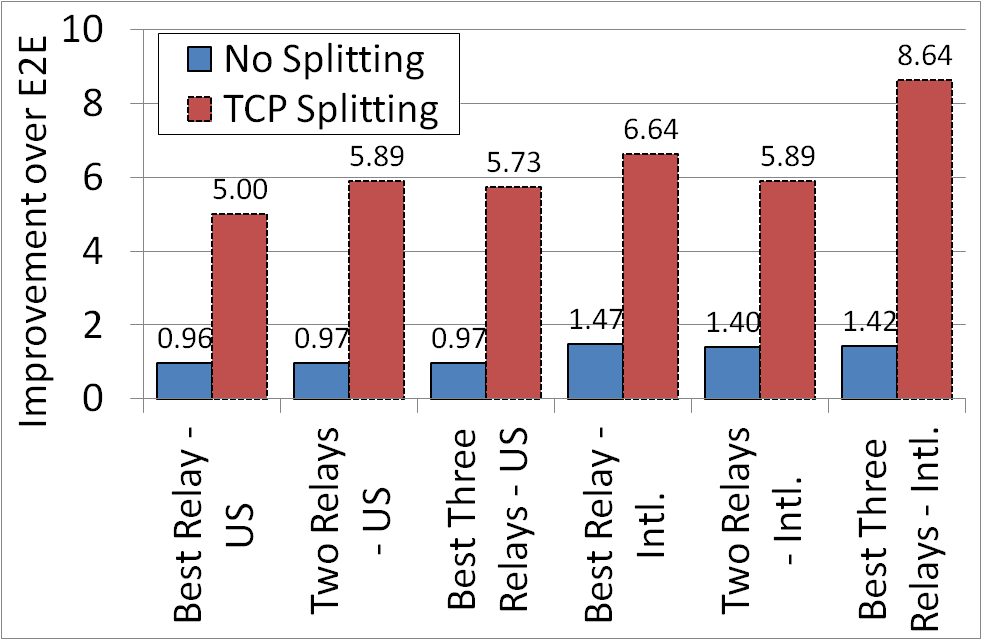
\includegraphics[width=0.97\textwidth,trim=2mm 2mm 2mm 2mm,clip]{figures/tcp_splitting_aws.png}
    \caption{Using AWS relays}
    \label{fig:must-split-aws}
\end{subfigure}
\begin{subfigure}{.32\textwidth}
  \centering
    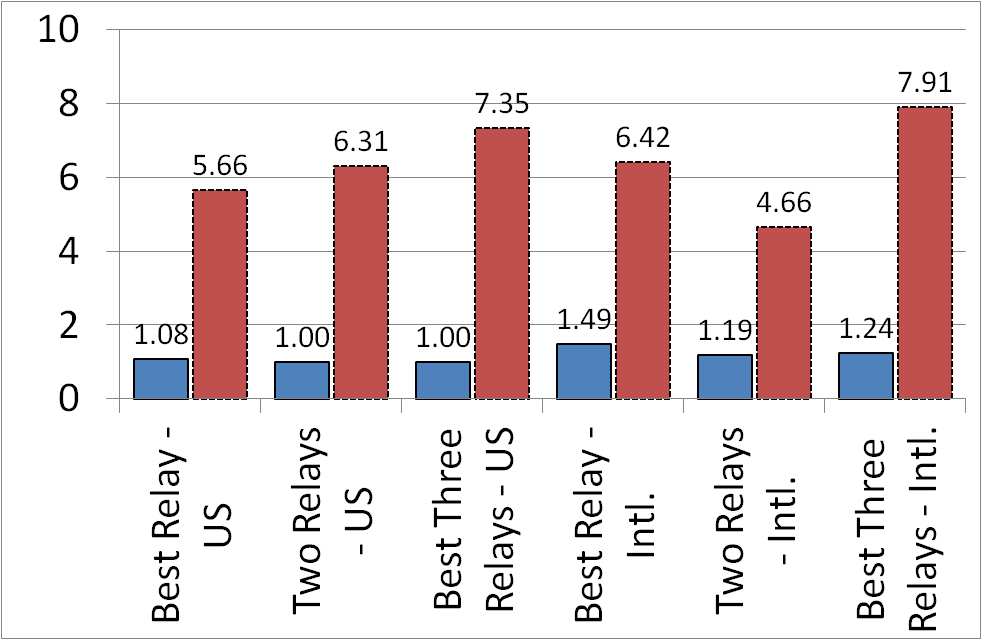
\includegraphics[width=0.97\textwidth,trim=2mm 2mm 2mm 2mm,clip]{figures/tcp_splitting_az.png}
    \caption{Using Azure relays}
    \label{fig:must-split-az}
\end{subfigure}
\begin{subfigure}{.32\textwidth}
  \centering
    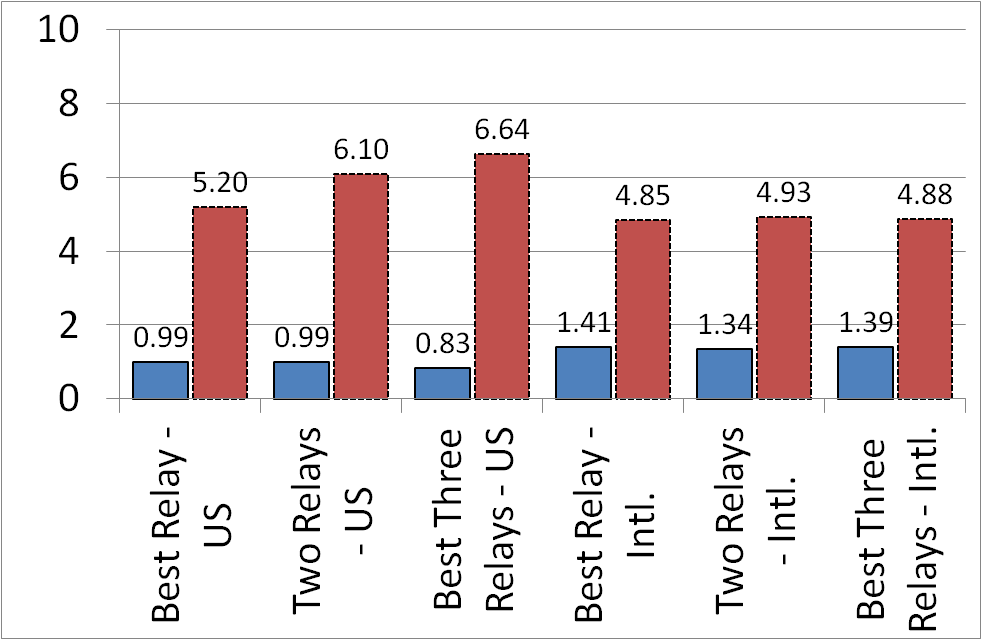
\includegraphics[width=0.97\textwidth,trim=2mm 2mm 2mm 2mm,clip]{figures/tcp_splitting_gcp.png}
    \caption{Using GCP relays}
    \label{fig:must-split-gcp}
\end{subfigure}
\caption{Evaluation of the benefits of (1) \textit{going through the cloud}; and (2) \textit{using TCP splitting}. \textbf{(1)} The left blue bars display the performance of \textit{going through the cloud without TCP splitting}. In the intra-US case, when sending a large file from New York to San Francisco, there is little performance change. For example, the best case is a 1.08$\times$ improvement with the best single relay in Azure, while the worst is the 0.83$\times$ performance in the three-relay GCP case. The international case between Mumbai and SF does display some improvement of about 40\%. \textbf{(2)} The right red bars display the performance of \textit{going through the cloud with TCP splitting}. The performance improvement is noticeably larger across all clouds. The best-single-relay and the simple-dual-relay experiments display some 5$\times$ improvement; the best-triple-relay experiments typically improve this further to some 6-8$\times$ improvements.
}
%TCP splitting is a must
\label{fig:must-split}
\end{figure*}

% \IK{References to related work should probably go to the Intro; move/delete this next paragraph?}
% {\small
% Previous studies~\cite{CRONets} suggested TCP splitting\AB{Did we elaborate on what this means and how we do it somewhere above?}\NR{Nope, I think we should put it in with the methodology portion} would improve performance. Our first goal was to quantify the affect of this feature across multiple scenarios. 
% We experimented using inter-continental routes as well as regional routes, and the three different clouds at our disposal.\AB{perhaps this should be included in the methodology section?}
% For brevity, we only show the benefits of splitting when default Cubic is used as the congestion control algorithm in the relay nodes, and compare it to simply routing through the cloud nodes using one, two or three relays on the cloud.
% }

\subsection{TCP Splitting is Crucial} 

We start by evaluating the benefits of 
\begin{inlinelist}
    \item \textit{going through the cloud} through one, two, or three relays,  instead of the regular fully-Internet-based E2E (end-to-end) route; and \item \textit{TCP splitting}.
\end{inlinelist} In all cases, the average bandwidth results are normalized by the average bandwidth in the E2E experiment.

%\autoref{fig:must-split-aws}--\autoref{fig:must-split-gcp} 
\autoref{fig:must-split} shows the results for two main scenarios: an internal US connection between the SF client and the NY server, and an international connection between the SF client and the Mumbai server. %It differentiates the benefits by considering different data delivery methods in all three clouds.\AB{not sure what the last sentence means.}

The main take-home messages are that (1) going through the cloud without TCP splitting is not particularly helpful; (2) TCP splitting remarkably accelerates download; (3) the simple two-relay placement and the best single relay provide comparable improvements over E2E download; (4) using three  relays can typically (for the proper choice of relays) strictly improve over the 2-relay strategy.
 %\IK{please check if you agree with the conclusions} \NR{@Aran, we didn't check all the 4 node options, right?}\AB{If you mean 4 relays - I only have one experiment with this setup. Why do you ask?}
 
Why does TCP splitting have such a positive effect on performance? We argue that the reasons are as follows. TCP's performance in steady-state is reciprocal to the RTT between the end-points~\cite{mathis1997}. Splitting the link between the end-points results in path-segments with shorter RTTs, and therefore better performance. Also, a shorter RTT enables much faster ramp-up of the transmission rate during TCP slow-start. Our experiments show that in the long-haul section of the path, TCP is in slow-start during the entire download period (\S\ref{subsec:quick-start}). Yet another reason is TCP's innate unfairness towards long RTT flows. Whenever the TCP flow competes with other flows on some bottleneck along the path, it is suppressed by flows with lower RTTs.



% performance of various data delivery alternatives for six different scenarios, \ie 
% using the same client-server pair, and different cloud providers for relay nodes. The client is the San Francisco client, and the server is in Mumbai (utilizing an international route).
% Each bar represents the gain of this routing option over the regular E2E option. For the single-relay and three-relay options, both with and without TCP splitting, we only show the gain of the best performing region out of all the regions used for each of these options.

%\IK{should we insert philosophical comments on the costs of  1 optimized vs 2 naive; or of splitting?}

%It is clear that for each hop-count variant we used the better option is to employ TCP splitting. This is also true for the regions not presented in \autoref{fig:must-split}. Using TCP-splitting either has the same or better performance than the same routing option without splitting.

% In \autoref{fig:must-split-gcp} and \autoref{fig:must-split-az} we see the same trend for the other cloud providers we used for the relay nodes.


\subsection{Finding the Best Relay is Hard} %\IK{feel free to have another title here}
%How Many Relays?} \IK{Or: ``What Relays?"}
%When using an overlay network, one may ask, how many relays are too many?
%We began by trying all the options for a single relay. In addition, we tested the simple heuristics of using the relays, one closest to the client, and the other closest the the server. Finally, we  tested adding the nodes that performed best as single relays to the formally mentioned two relays. \NR{Per IK's changes to the Methodology, do we want to remove this paragraph?}



%Let's focus on the cloud relay options of \autoref{fig:must-split}. It is not clear that we have to either pay for two relays, 

\begin{figure}
  \centering
    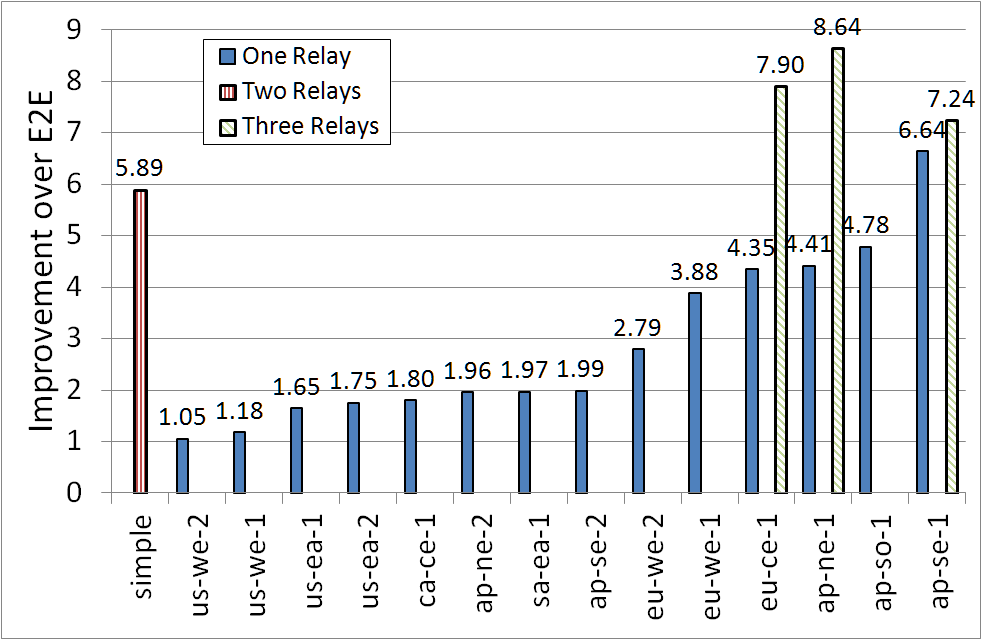
\includegraphics[width=\columnwidth,trim=2mm 2mm 2mm 2mm,clip]{figures/hops.png}
    \caption{One, two and three relays when using  TCP splitting in AWS for the Mumbai-SF international setting. (1)~The first striped red bar shows the performance of the simple unoptimized two-relay placement at the nodes that are closest to the client and the server. (2)~Next, the 14 blue bars show all the options for a single-relay option. The best option is ap-se-1 with a normalized performance of 6.64$\times$, above the two-relay option. However, all other single-relay options have a lower performance, and the    median option gets 1.99$\times$, \ie only 30\% of the best performance. (3)~Finally, the three green bars show a few options for the middle relay in the three-relay method, given the simple two-relay options at the extremities; \eg eu-ce-1 shows the performance of consecutively going through (us-we-1$\to$eu-ce-1$\to$ap-so-1). The best option is ap-ne-1 with an 8.64$\times$ performance.} 
    \label{fig:how-many-hops-aws}
\end{figure}

How hard is it to identify the best \emph{single} relay? \autoref{fig:how-many-hops-aws}
%After considering Figure~\ref{fig:must-split}, one might be inclined to think that a single relay might provide better performance than the two relays, chosen by using our simple approach. Figure~\ref{fig:how-many-hops-aws} 
extends \autoref{fig:must-split-aws}, showing the results for all the relay options tested in AWS using TCP splitting in the international case. 
We learn that (1) all but one relay perform \emph{worse} than the simple two-relay option; (2) the \emph{best} single relay (ap-se-1, \ie ap-southeast-1 in Singapore) indeed performs better than our simple two-relay approach, but this relay is neither the closest to the client, nor the closest to the server, nor the (geographically) closest to the mid-point. 

This suggests that determining the identity of the best single relay to use is nontrivial as this relay seems to have no obvious characteristics. While \autoref{fig:how-many-hops-aws} shows results for relays in AWS, similar results were observed when using GCP and Azure.

\subsection{TCP is Enough} 
%While the effects of congestion control in overlay networks have been discussed before(~\cite{CRONets}, \NR{are there any more?}), much is left unknown.
We tested the performance of the default TCP Cubic against the recently proposed BBR with the same international setting on AWS using TCP splitting. Note that we only deployed BBR  on the relay nodes and not at the end-points.
%The results of our experimentation across all scenarios yielded similar results. 
As shown in \autoref{fig:aggressive},
%showcases representative results. %The experiment setting is a personal computer client in the San Francisco area (SF), relays in AWS, and a web server in Mumbai. As can be seen in the figure, 
BBR did not achieve better performance than default TCP.
%BBR was activated in all the relay nodes. It did not help in achieving better performance.

% \begin{figure}
%   \centering
%     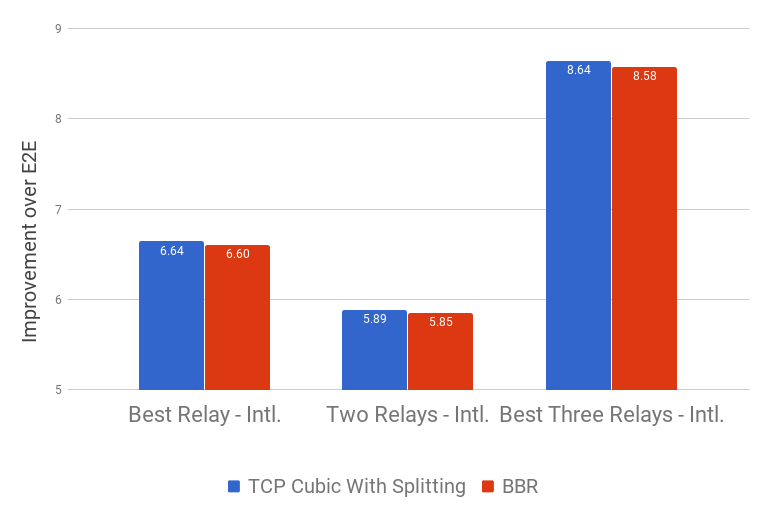
\includegraphics[width=0.47\textwidth]{figures/bbr.png}
%     \caption{TCP Cubic vs. BBR, using AWS relays}
%     \label{fig:tcp-vs-bbr}
% \end{figure}
%\AB{Do we want a CDF of BBR/TCP over all experiments?}


\subsection{Using Quick-Start TCP Pays Off}\label{subsec:quick-start}
%While the effects of congestion control in overlay networks have been discussed before(~\cite{CRONets}, \NR{are there any more?}), much is left unknown. We therefor conducted experiments on our relay machines in multiple scenarios, testing TCP without splitting, TCP Cubic with splitting, BBR~\cite{BBR} and aggressive TCP. \NR{@AB, can you fill our the details of the aggressive TCP?} 
\autoref{fig:aggressive} illustrates the impact of using Quick-Start TCP Cubic  instead of TCP Cubic or BBR.
%, in the same experimental settings as in \autoref{fig:tcp-vs-bbr}
We observe that (1) Quick-Start TCP significantly improves upon TCP Cubic and BBR, and (2) this improvement is particularly large with two or three relays. We hypothesize that their performance gain is similar because the main benefit of using the third (middle) relay is in reducing the impact of the slow-start phase by reducing the RTT, and Quick-Start TCP avoids slow-start altogether.

%\IK{here we need to explain what happens for (a) other clouds, (b) US. For instance, is it just a coincindence that perf(2 relays)=perf(3 relays)?}


% Next, we tested the performance of aggressive TCP.
% While the results varied from cloud provider to another, a trend did emerge: aggressive TCP yielded better, and in most cases using two or three relays, much better results than TCP Cubic (or BBR). In the experiment depicted in Figure~\ref{fig:aggressive} we used Azure nodes for relays.

We were wondering whether Quick-Start Cubic is too aggressive and unfair towards other regular TCP flows. By essentially skipping the slow-start phase of TCP, even though we keep the connection remainder unchanged, aren't we just hogging the link and exploiting a loophole
that cloud providers should soon close?
\autoref{fig:agg-vs-cubic} looks at the per-byte download time of our large file in the cloud. We learn that (1) the average throughput is clearly higher for the Quick-Start TCP, as expected from \autoref{fig:aggressive}; but (2) this is mainly because TCP cubic tends to operate in a sporadic bursty manner in its slow-start, by first waiting for a full RTT for a bunch of ACKs to arrive back to the server, then sending bursts of packets to catch up. When zooming on the TCP-cubic bursts, its slope surprised us by being higher than for the Quick-Start TCP, \ie it is \textit{more} aggressive because of this catching up. 


%Th e effects of congestion control in overlay networks have received some attention in previous studies ( \NR{are there any more?}). We have decided to conduct a

\begin{figure}[!t]
  \centering
    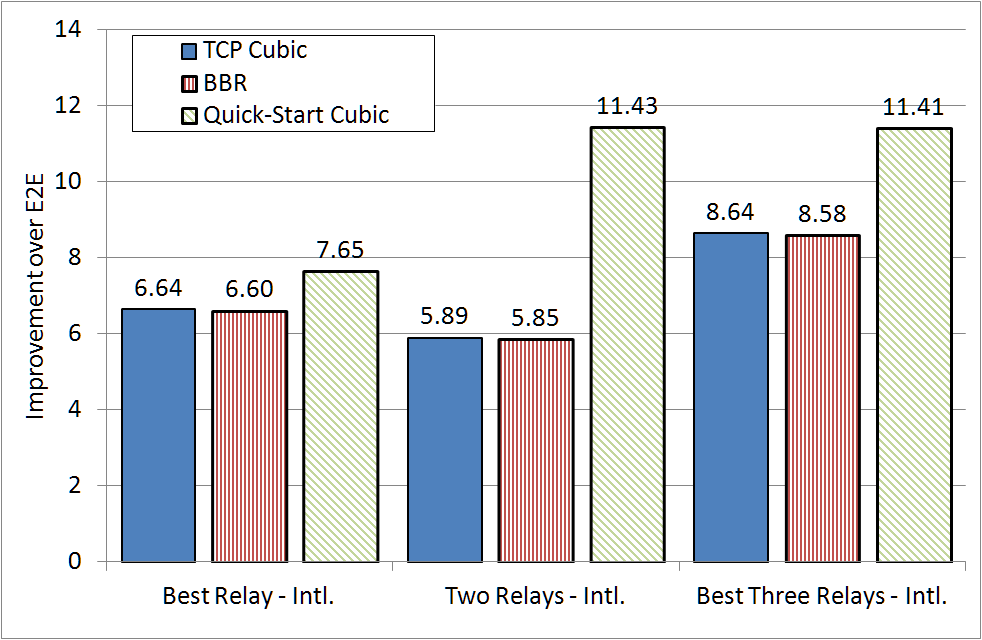
\includegraphics[width=0.47\textwidth,trim=2mm 2mm 2mm 2mm,clip]{figures/aggressive.png}
    \caption{Impact of Quick-Start TCP demonstrated using the Mumbai-SF international transmission of a large file with TCP splitting over AWS. In all three cases of best-single, simple-double and best-triple relays, Quick-Start TCP achieves remarkably higher efficiency. In the last two cases, it achieves an impressive 11.4$\times$ improvement over E2E.
   }
    \label{fig:aggressive}
\end{figure}

\begin{figure}[!t]
  \centering
    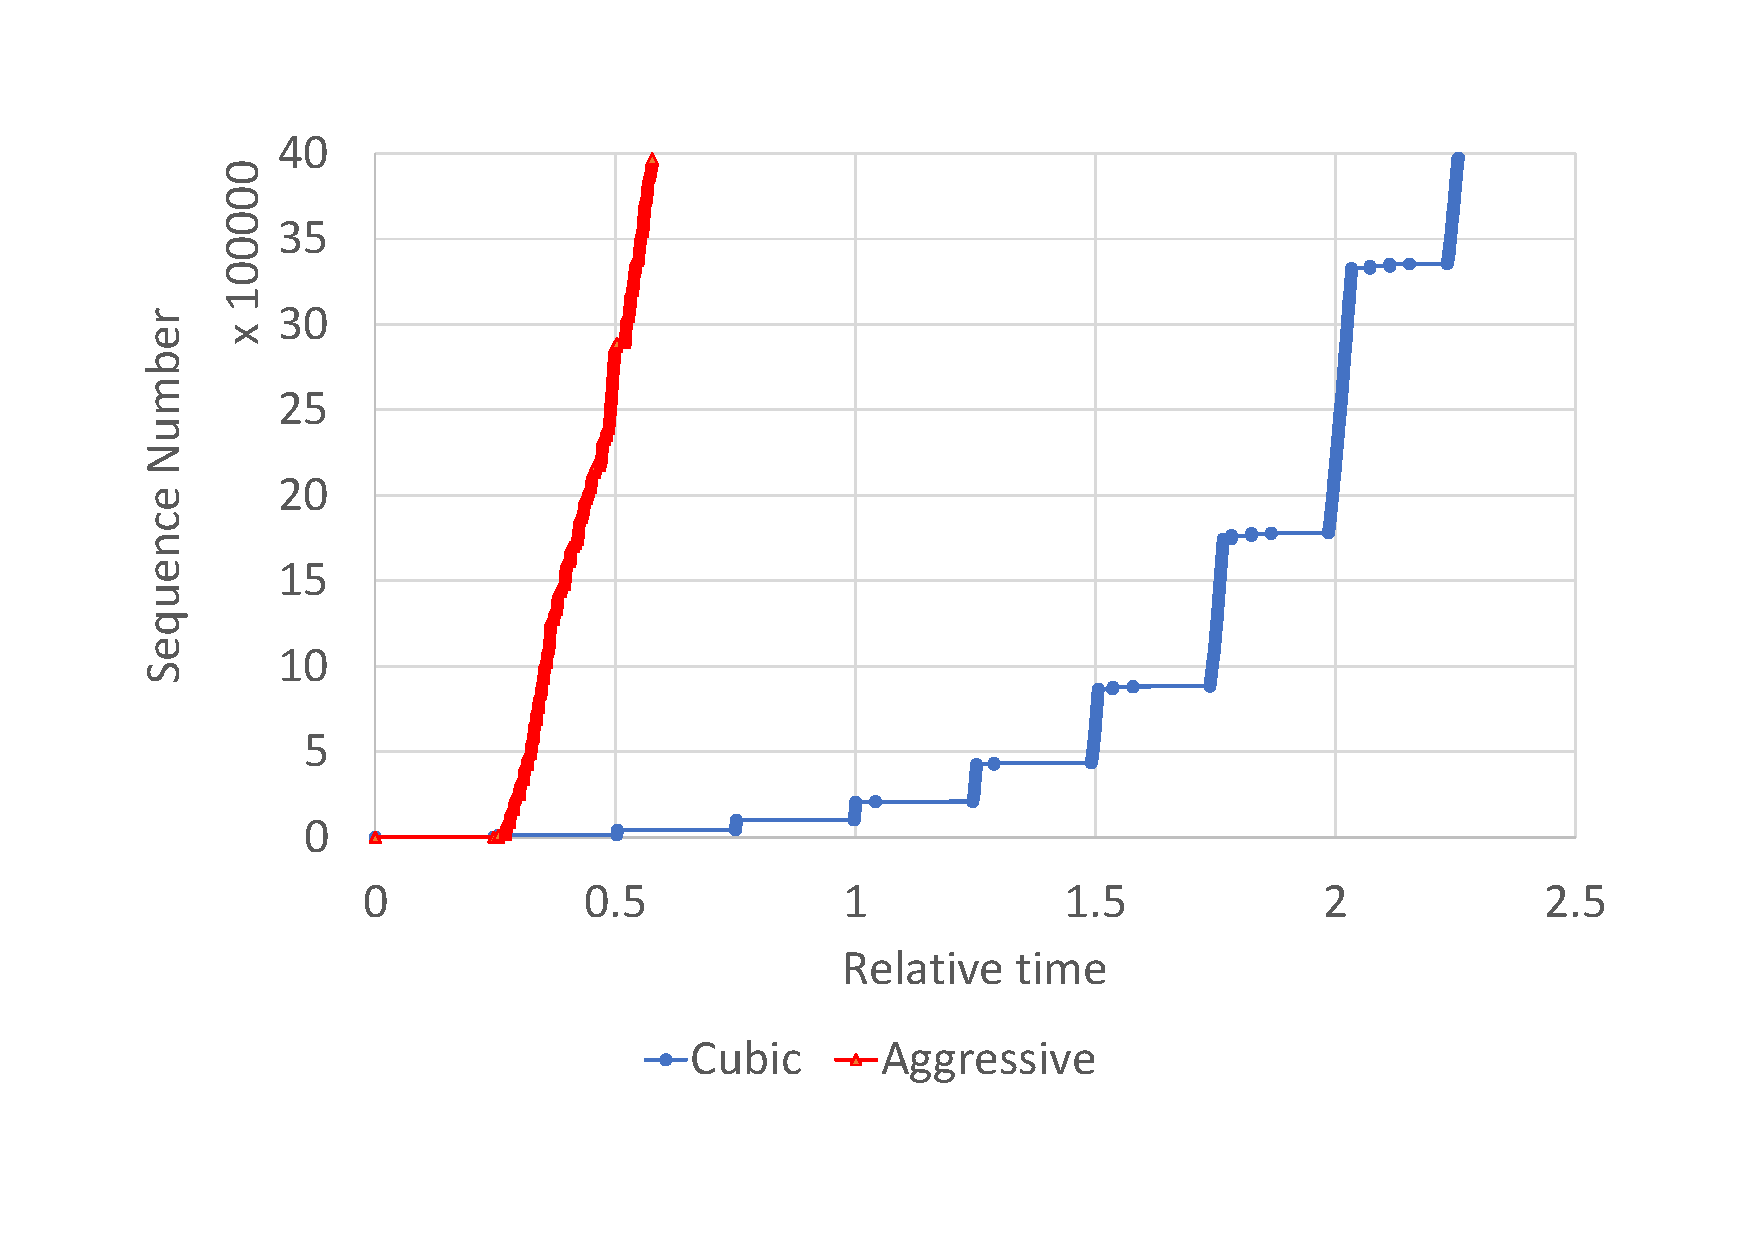
\includegraphics[width=0.47\textwidth,trim=2mm 2mm 2mm 2mm,clip]{figures/CubicVsAggressive-seq}
    \caption{Per-byte look at the flow between \rs and \rc, as captured on \rc. The graphs depict the sequence number received \vs relative time (to the beginning of the TCP connection). The transmission rate during the bursts in the default cubic option is 260 MBps while it is only 110 Mbps when the Quick-Start option is used. However, since Quick-Start avoids slow-start, its overall download time is much shorter.  
    %Why aggression pays off
    }
    \label{fig:agg-vs-cubic}
\end{figure}

% \begin{figure}[t]
%   \centering
%     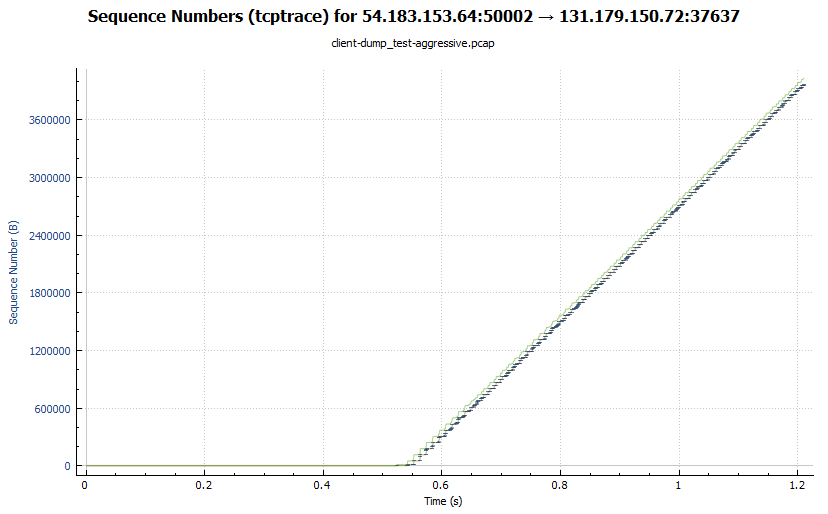
\includegraphics[width=0.47\textwidth]{figures/client-aggressive-tcptrace}
%     \caption{Client with limited rwin - with a close relay and aggressive TCP \AB{should this stay or go?}}
%     \label{fig:close-to-poor-client-benefit-aggressive}
% \end{figure}


\subsection{File Size Matters}
%\label{sec:file-sizes}
The previously-presented results are for large file downloads. What about small files? \autoref{fig:small-file} illustrates how our experimental results for small files exhibit similar trends in the international case: TCP splitting is better, and Quick-Start TCP helps. However, in the US case, in contrast to the large files, even the best results provide no improvement beyond simple E2E delivery. 

\begin{figure}[t]
  \centering
    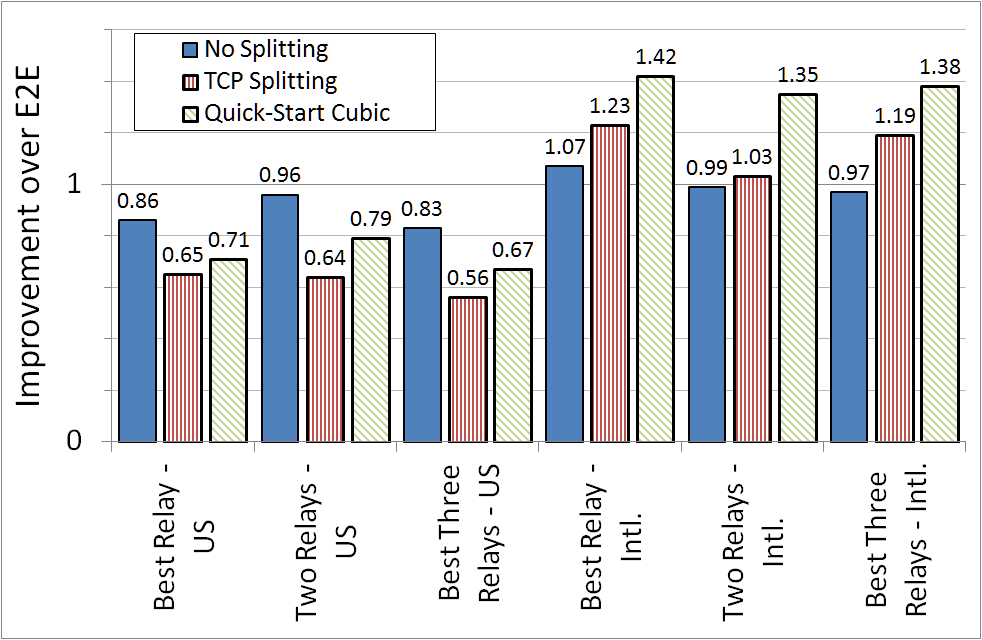
\includegraphics[width=0.47\textwidth,trim=2mm 2mm 2mm 2mm,clip]{figures/small_file}
    \caption{Small-file results using AWS relays. In the international Mumbai-SF case, TCP splitting performs better than non-splitting, and Quick-Start TCP further improves performance. However, in the US case, the best  results with splitting are still about 30\% lower than E2E.}
    \label{fig:small-file}
\end{figure}

\subsection{Is RTT a Good Proxy for Performance?}

In contrast to measuring bandwidth, measuring latency (in terms of RTT) is simple. When is RTT a good proxy for performance, in terms of download completion time?

\noindent{\bf Without TCP splitting.} When TCP is \emph{not} split, end-to-end RTT is a good proxy for download completion time: the shorter the RTT, the shorter the download. We used RTT measurements to estimate the improvement of different routing strategies over E2E by calculating the ratio between the E2E RTT and the RTT of the tested route. \autoref{fig:rtt-estimate-nat-1hop} plots the correlation between our estimator and the actual performance gain. % for single-relay (no TCP splitting).

\noindent{\bf With TCP splitting.} When TCP splitting is used, with Cubic as the congestion control algorithm, an RTT-measurements-based estimator succeeded in predicting the performance gain of the 3-relay method over the 2-relay method. This is accomplished by calculating the ratio of the RTT between \rc and \rs and the maximum RTT of the segments of the route through the third node used between them. Namely, if $\rtt(\rc,\rs)$ is the RTT between \rc and \rs, $\rtt(\rc,\rmid)$ is the RTT between \rc and the middle relay, and $\rtt(\rmid,\rs)$ is the RTT between \rs and the middle relay, we estimate that using this third relay would improve download time by 
\[
\frac{\rtt(\rc,\rs)}{\max(\rtt(\rc,\rmid),\rtt(\rmid,\rs))}
\]
compared to using the two-relay route using \rc and \rs only.
The reasoning behind this estimator is that when splitting is used, the throughput is limited by the slowest segment of the route. \autoref{fig:rtt-estimate-ssh-3hop} depicts the correlation between this estimator and the actual gain of the 3-relay method over the 2-relay method (both with TCP splitting at each relay).

Motivated by the relative accuracy of this estimator, we used RTT measurements to predict which 4-relay route would fare best when using TCP splitting and Cubic as the congestion control protocol. The 4-relay route achieved an improvement of 8.57$\times$, \ie higher than the 7.38$\times$ improvement achieved with the 3-relay route calculated with min-max RTT between \rc and \rs. 
%In \autoref{fig:4-relay-route-cubic} we compare the route found using this method to the best 3-relay route and the 2-relay method. 
 
We point out that, in contrast to the above results, this estimator fails to provide good results for the single relay with TCP splitting strategy, possibly because as RTTs get higher the impact of congestion and loss rate becomes more significant.
%\AB{Do we want a section about using RTT as an estimator of TCP performance?} \IK{please give us a plot draft so we can decide what we have to answer; this can join the lesson (1) of Figure 2, or the part of Figure 3.}


\begin{figure}[t]
  \centering
  
    \begin{subfigure}{0.47\columnwidth}
  \centering
  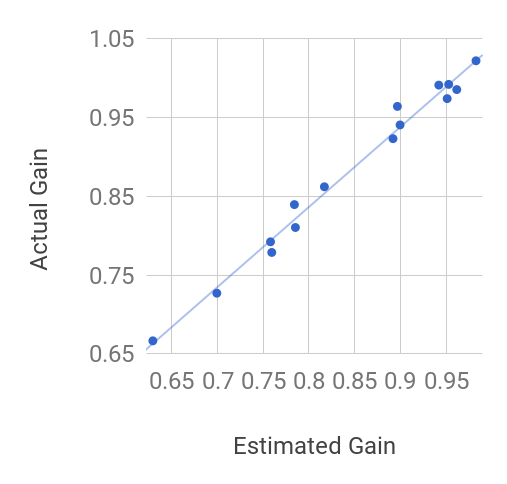
\includegraphics[width=\columnwidth]{figures/gainEstimateVsActual-nat-1hop-newer}
    \caption{}
    \label{fig:rtt-estimate-nat-1hop}
\end{subfigure} \hfill
\begin{subfigure}{0.47\columnwidth}
  \centering
  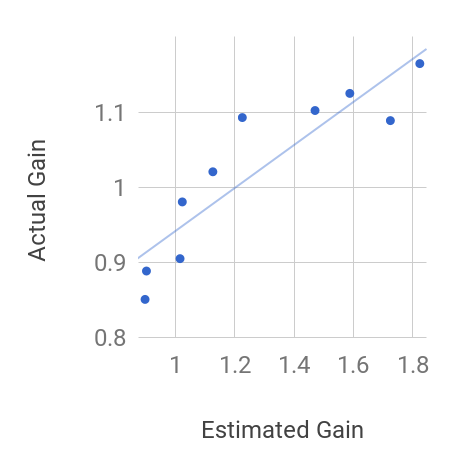
\includegraphics[width=\columnwidth]{figures/gainEstimateVsActual-ssh-3hop-newer}
    \caption{} \label{fig:rtt-estimate-ssh-3hop}
\end{subfigure}
    \caption{Performance gain estimates \vs actual gain of \textbf{(a)} the single relay method without splitting; and \textbf{(b)} the 3 relay setup with splitting.}
\end{figure}

%\begin{figure}
%  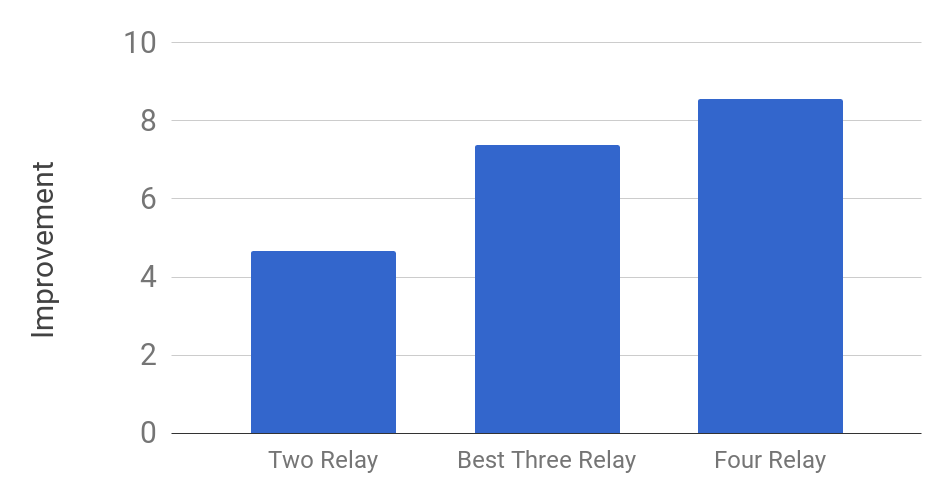
\includegraphics[width=0.47\textwidth]{figures/4relaysVs2and3}
%    \caption{Results of a 4-relay route with TCP splitting using TCP cubic. 4-relay route chosen as min-max route between \rc and \rs using RTT measurements. The graph depicts improvement over the E2E method when using SF as client, Mumbai as server and using cloud nodes on Azure. The nodes used in the 4-relay route are westus$\to$japaneast$\to$southeastasia$\to$westindia.}
%    \label{fig:4-relay-route-cubic}
%\end{figure}


\subsection{Mixing Clouds}

We also tested whether routes traversing different clouds can produce better results. To this end we rerun the 2-relay and 3-relay experiments (with TCP splitting) using the SF client and Mumbai server with \rc on AWS and \rs on Azure. We compared performance to that of the same strategies with AWS relays only. Our preliminary results show that mixing clouds was indeed beneficial in some of the evaluated scenarios--- specifically, when Quick-Start Cubic was used and/or when three relays were used (with either Cubic or Quick-Start Cubic). 

% In case we do have room for the graph:
% This is exemplified by the sequence number graphs we present in \autoref{fig:close-to-poor-client-benefit}

% \begin{figure}[t]
%   \centering
%     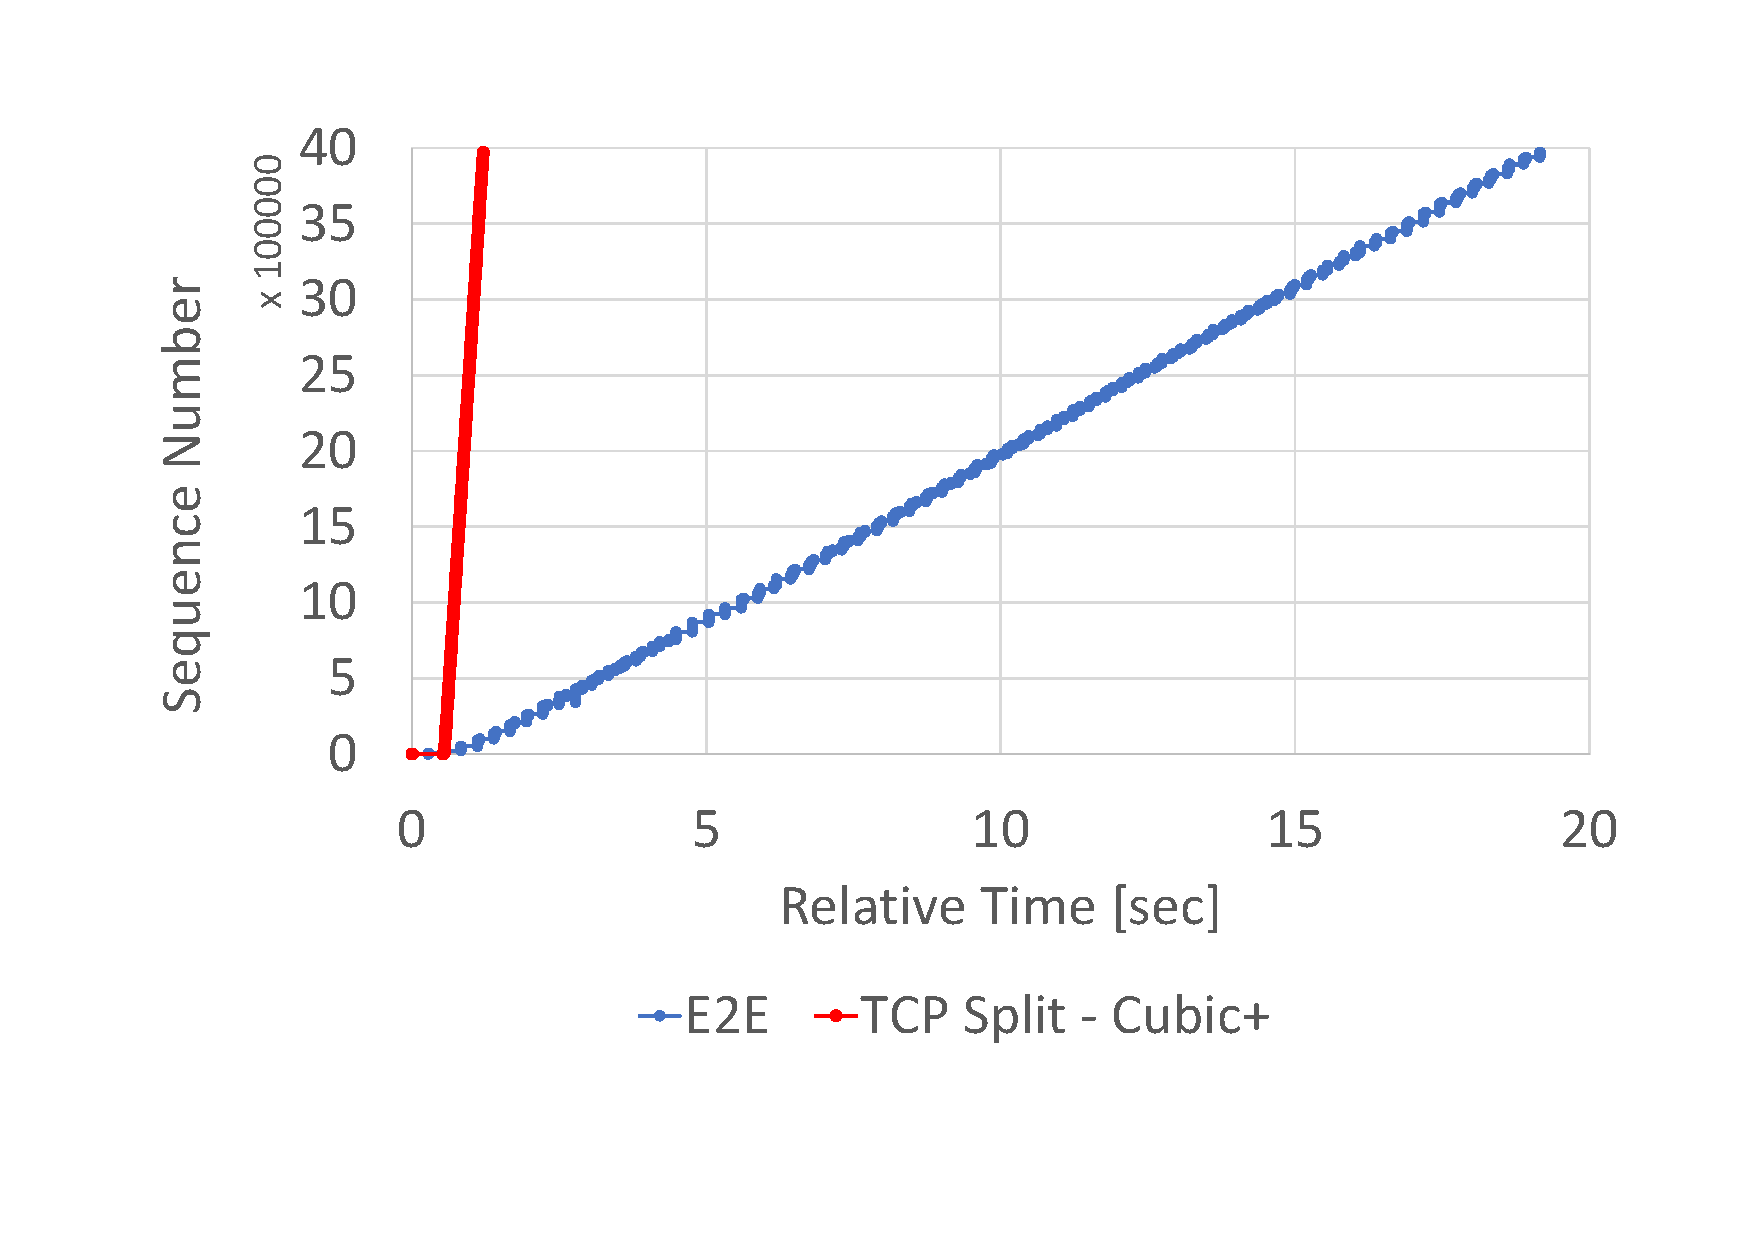
\includegraphics[width=0.47\textwidth]{figures/client-e2eVsAggressive}
%     \caption{Client with limited rwin. The receive window and the RTT set the throughput. This graph compares the sequence number of the first byte in each received packet between the E2E method and the 2-relay TCP split using Quick Start Cubic}
%     \label{fig:close-to-poor-client-benefit}
% \end{figure}

\section{Related Work}

\EZ{\cite{le2016understanding} is a 5 pages workshop (CAN'16) from IBM's group (CRONets). 
They make very strong claims: (1) the bottleneck is not the overlay but the Internet path to get to the cloud (2) simple forwarding (without a proxy/split) gains only 13\% (3) "multi-hop indirection" (their terminology) do not add to single-hop.
Comparison to us: (1) worked with one cloud only (IBM) (2) their single server is inside their cloud (3) never really checked multi-hop (4) the clients are located in IBM's branches which is not exactly "outside the overlay" (5) do not mention congestion control even once.}

\T{Internet overlays.} The idea of overlay networking on top of the Internet dates back almost two decades~\cite{old-overlay-1, old-overlay-2, RON}. Many studies established that the default BGP path between two end-points is often inferior to an alternate path traversing an overlay network~\cite{old-overlay-1, old-overlay-2, RON, akamai-2, akamai-3, akamai-4}. Akamai's SureRoute service relies on such an Internet overlay network.

\T{Cloud overlays.} Recently, overlay networking through the \emph{cloud} has received attention from both researchers (e.g.,~\cite{CRONets}) and practitioners (e.g.,~\cite{teridion}). CRONets~\cite{CRONets} leverages a \emph{single} cloud relay with TCP splitting for data delivery. Our experimentation with a broad spectrum of routing and congestion control schemes for cloudified data delivery, suggests that cloud overlays can provide significantly higher performance than that achievable using only a single relay.
% \EZ{I think we can stop here. Why would we like to present more of their findings?} and show that up to 50\% of the paths do not improve their throughput by going to the cloud when TCP splitting is disabled. 
%provides a strong argument in favor of this transit point. However, unlike in the \name overlay network that relies on a full routing solution through the cloud, CRONets only relies on a single-hop transit through the cloud. 
%However, they neither consider more than one cloud relay, nor accelerated solutions like our quick-start TCP. \IK{How can we make this stronger?}
%\EZ{Instead, we can use their own future-work statement. Something like this} 

\T{Cloud-based content delivery.} The use of an HTTP proxy~\cite{cgn2017} in static AWS locations was shown to reduce webpage load times by half, when accessing remote websites. Cloud-based mobile browsing~\cite{zhao2011reducing,wang2013accelerating} is a common technique for reducing cellular costs and decreasing download times.

\T{Cloud connectivity and performance.} \cite{one-hop} shows that some 60\% of end-user prefixes are within one-AS-hop from GCP (Google Cloud Platform). A different study~\cite{cgn2017} established that AWS has at least one node within a median RTT of merely 4.8~ms from servers hosting the top 10k most popular Web sites. \cite{unusual} shows that modern clouds have unusual internal routing structures that are hard to infer and CLAudit \cite{multidimensional} points out the increasing reliability of cloud latency. 

\T{TCP Splitting.} Several papers considered TCP splitting as a way to improve TCP's performance, \eg to overcome different link characteristics~ \cite{Kopparty2002} (wired and wireless), to compensate for very long RTTs in satellite links \cite{luglio2004}, and to reduce search query latency~\cite{pathak2010measuring}. 
Pucha and Hu explore TCP overlay \cite{pucha2005overlay, pucha2005slot}. 

% Teridion~\cite{teridion} has recently announced it is using cloud overlay networks as an alternative to support the acceleration of dynamic content in the context of CDN networks. %\IK{Can we weaken this first sentence? If not, how strong is our novelty?} \IC{I don't think companies that do not disclose how they solve these problems are a big  
% %dynamic content in the context of CDN networks. 
% % Teridion seems to implement an overlay network over the public cloud that optimizes routes and TCP performance to carry a CDN-like acceleration for dynamic web and SaaS services. 
% The Teridion network accelerates the downloads and Web interaction for service providers (\eg Box, Egnyte) for dynamic transactions or private content that traditional CDN technology cannot support. Therefore, unlike CLEAN, % that provides full corporate connectivity over a business-type Internet, 
% the Teridion network does not provide connectivity between branch offices, datacenters and mobile users, has a single destination per customer, and does not provide any secure VPN connections or any reliability guarantees.  Unfortunately, they have also not disclosed the details of their internal architecture. 

% Incidentally, Akamai~\cite{akamai} has also introduced a new service termed ``Dynamic Site Acceleration" that is based on TCP split and optimal routing between Akamai edge servers. However, they are not using the public clouds.  





%\T{Resilient overlay networks}. The Resilient Overlay Network (RON)~\cite{RON} establishes an overlay network that can quickly restore communication following failures that disconnect Internet paths. The authors argue that in practical Internet environments, RON only takes tens of seconds for the routing algorithms to detect and reroute around failures. RON is implemented in several locations on top of private servers. It uses distributed link-state routing algorithms between these servers. Since RON is an early work (2001), it does not take advantage of the public cloud compute and high-speed networking infrastructure and guarantees as well as of SDN-based architectures. As the main goal of RON is to circumvent Internet failures, it also does not split TCP connections or deal with QoS and security issues related with a global business Internet.

%\T{Leased backbone.} Additional companies address the relocation of corporate WANs to a network service through the introduction of a specialized backbone network rather than using the public clouds, \eg Aryaka~\cite{aryaka}, Cato Networks~\cite{cato} and Virtela~\cite{virtela}. 

%\T{SD-WAN.} A large number of companies is solving the problem of backhauled Internet traffic over expensive corporate WANs by downloading and uploading Internet traffic from the branch office directly to the Internet, without passing through the corporate secure gateway. Since corporations insist that this traffic must be secured and inspected, the firewall and other security functions are distributed to the branch offices and managed centrally. Our \name network can help provide a better and more reliable performance to this Internet-based traffic.

%\T{Cloud destination.} FootPrint~\cite{footprint} provides an integrated system for jointly allocating the right cloud proxy and datacenter to each client as well as routing through the best route. Its goal is to access a cloud datacenter destination by using the WAN, while the goal of \name is to build an overlay on the cloud to replace the corporate WAN and therefore to exploit the cloud inter-connection network, even when accessing a SaaS website.

% \T{Full network path.} ARROW~\cite{arrow} allows users to configure reliable
% and secure end-to-end paths through a set of different providers. 
% %In contrast, by controlling all links within its network, \name enables a uniform security guarantee that can easily be strengthened.
% In addition, \cite{nira} suggests a new Internet routing architecture (NIRA) that gives a user the ability to choose the sequence of providers his packets take. The goal of \name, in contrast, is to obtain a single cloud overlay provider.



\section{Conclusion}

We initiated the systematic exploration of cloudified data delivery and presented initial results suggesting that optimization of performance should be viewed through the congestion-control lens.  We view cloudified data delivery as a promising direction for overcoming the inefficiencies of today's routing (BGP) and congestion control (TCP) protocols. We thus argue that tapping the full potential of this approach is of great importance. 

Our results leave many important questions wide open. We discuss some of these below.

\T{Cloudified data delivery vs. state-of-the-art end-to-end congestion control.} Recent studies claim to improve performance by an order of magnitude by employing better congestion control protocols end-to-end~\cite{PCC}. How does this compare to cloudified data delivery? Could routing through the cloud be redundant?

\T{Modeling the cloud.} Though we provided intuitions for our empirical results, the root causes underlying our results remain hidden. We believe that more thought should be given to generating (from empirical observations) models of the cloud(s) that can provide insights into its inner workings.

\T{Is Quick-Start TCP too aggressive?} Our results (\S\ref{subsec:quick-start}) provide partial evidence that Quick-Start TCP is not necessarily more aggressive to other connections than regular TCP. Providing better empirical support of this claim is crucial, as better performance for cloud users should not (arguably) come at the cost of harming others.

%\IK{Copying here our comment:} \IK{Note that I commented the parts about cloud servers following your comments; please uncomment if we do intend to use cloud servers.} \NR{We used them in my experimentation, but didn't mention these yet. Do we want to? Maybe in the Future Work section?}
%\AB{Add sth about utilizing TCP fast open (\url{https://tools.ietf.org/html/rfc7413}, \url{https://www1.icsi.berkeley.edu/~barath/papers/tfo-conext11.pdf}) to reduce another RTT from the download time - might be the thing that makes 2hop with split better than e2e even for short files on short routes }


% \iffalse
% Optimizing performance \emph{within} an organizational network has been the subject of extensive attention, as evidenced by the many studies on performance optimization in datacenters~\cite{jupiter-rising,DBLP:conf/nsdi/SinglaGK14}, between datacenters~\cite{I-DC-TE}, in ISP networks~\cite{ISP-TEa,ISP-TEb}, and beyond. Optimizing routing across organizational networks is much less explored in comparison. One reason for this discrepancy is that introducing innovation into an organizational network is significantly easier than realising changes to the Internet that rely on the cooperation of many independently-administered organizations across multiple continents. We elaborate below several relevant threads of past research.

% \vspace{0.1in}\noindent{\bf Interdomain traffic engineering~\cite{IDR-TEa,IDR-TEb}.} As discussed above, BGP route-selection is based on network-operator-specified (static) local preferences over routes. Traditional traffic engineering with BGP thus translates to configuring local preferences over routes in a manner that efficiently splits an organization's outgoing traffic between its outgoing communication links. Researchers in this area proposed guidelines for BGP traffic engineering~\cite{IDR-TEb}. An online learning approach to BGP traffic engineering is presented in~\cite{IDR-TEa}.

% \vspace{0.1in}\noindent{\bf Software-defined Internet eXchange Points (IXPs)~\cite{SDX,SDXb}.} An interesting approach to optimizing traffic flow between organizations is focused on Internet eXchange Points (IXPs). An IXP provides a physical infrastructure through which organizations can directly peer. Today's largest IXPs provide this service to hundreds of organizations, and are thus a natural candidate for introducing innovation into inter-organization interconnection. Recent studies aim to bring the merits of Software Defined Networking (SDN) to the IXP context~\cite{SDX,SDXb}.

% \vspace{0.1in}\noindent{\bf End-to-end performance optimization~\cite{PCC,BBR}.} Much attention has been devoted to improving end-to-end performance on the Internet through changes to the communication end-points. A prominent and timely research direction is this context is replacing TCP congestion control with better-performance protocols~\cite{PCC,BBR}. Results along these lines demonstrate that improving upon TCP can result in very significant (over 5x-10x) improvement in performance. 
% \fi


%ACK
%Chen, Shay, Sujata

\bibliographystyle{abbrv}
\begin{small}
\bibliography{mybib,overlaybib}
\end{small}

%\bibliographystyle{plain}
%%\bibliography{abb,ultimate}

%\newpages

\end{document}